\begin{center}
	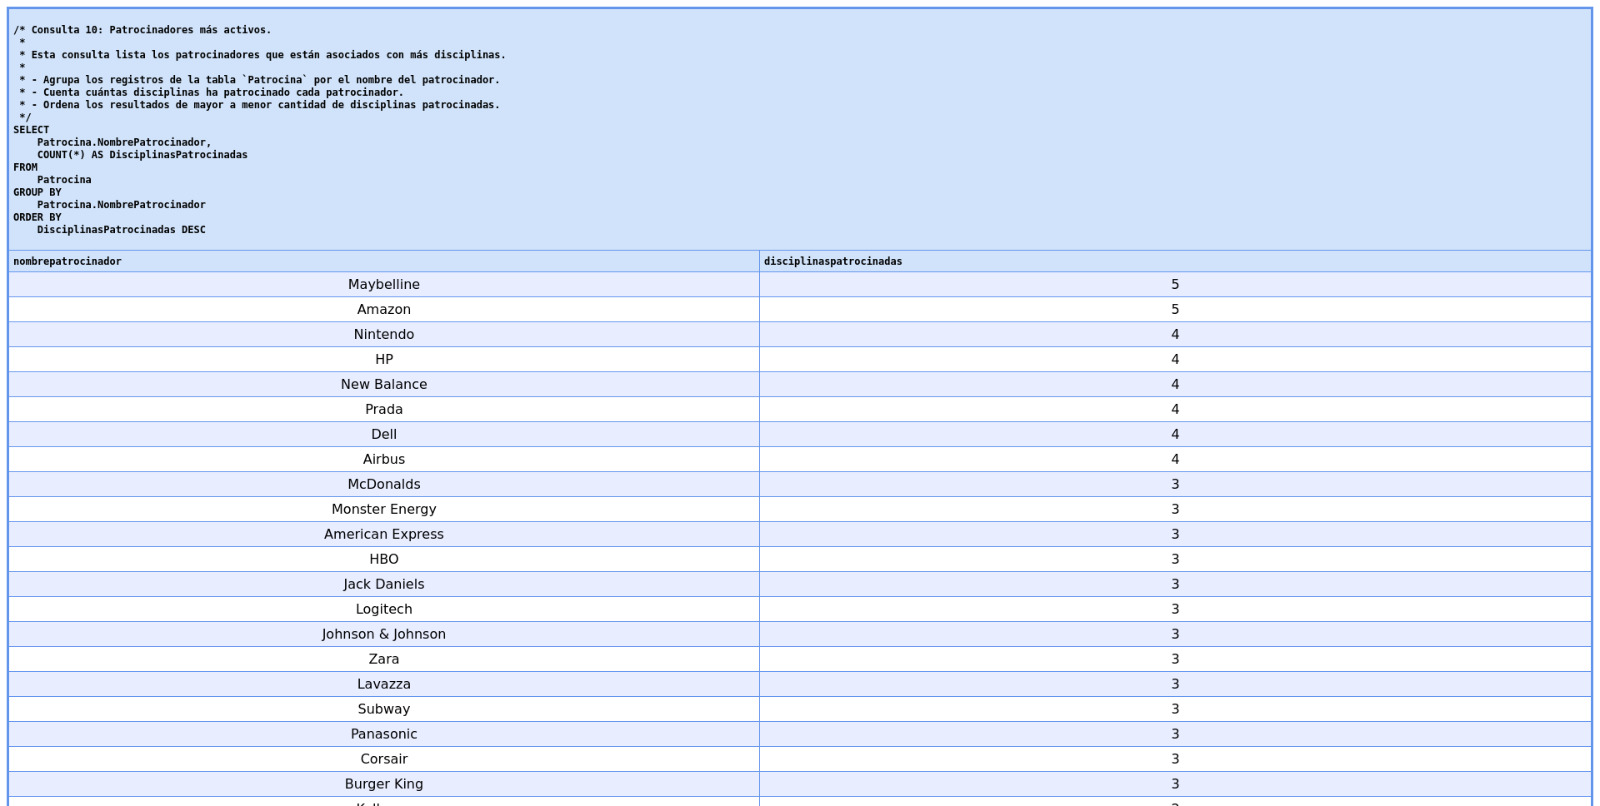
\includegraphics[width=16.5cm]{resources/Chapters/Consultas/Imagenes/Consulta10.jpg} 
	
	Consulta 10. Patrocinadores más activos. 
\end{center}

\textbf{Propósito de la consulta}

La consulta tiene como objetivo identificar a los patrocinadores más activos, es decir, aquellos que están asociados con la mayor cantidad de disciplinas patrocinadas. Los resultados se ordenan de mayor a menor según el número de disciplinas patrocinadas.

\textbf{Desglose de la consulta}

\begin{itemize} \item \textbf{Selección de columnas (\texttt{SELECT}):} \begin{itemize} \item \texttt{Patrocina.NombrePatrocinador}: Nombre del patrocinador, que identifica de forma única a cada entidad patrocinadora. \item \texttt{COUNT(*) AS DisciplinasPatrocinadas}: Cuenta el número total de disciplinas patrocinadas por cada patrocinador. \end{itemize}
	
	\item \textbf{Tabla involucrada (\texttt{FROM}):} \begin{itemize} \item \texttt{Patrocina}: Tabla que almacena la relación entre patrocinadores y disciplinas patrocinadas. \end{itemize}
	
	\item \textbf{Agrupación de resultados (\texttt{GROUP BY}):} \begin{itemize} \item \texttt{Patrocina.NombrePatrocinador}: Agrupa los registros por el nombre del patrocinador para calcular cuántas disciplinas ha patrocinado cada uno. \end{itemize}
	
	\item \textbf{Ordenamiento de resultados (\texttt{ORDER BY}):} \begin{itemize} \item Los resultados se ordenan por \texttt{DisciplinasPatrocinadas} en orden descendente (\texttt{DESC}), de modo que los patrocinadores más activos aparezcan primero. \end{itemize} \end{itemize}

\textbf{Análisis detallado}

\begin{itemize} \item \textbf{Relación entre patrocinadores y disciplinas:} \begin{itemize} \item La tabla \texttt{Patrocina} registra las asociaciones entre los patrocinadores y las disciplinas que apoyan, lo que permite calcular la cantidad de disciplinas patrocinadas por cada patrocinador. \end{itemize}
	
	\item \textbf{Uso de la función agregada \texttt{COUNT}:} \begin{itemize} \item \texttt{COUNT(*)} cuenta el número total de registros asociados con cada patrocinador, lo que representa el número de disciplinas que han patrocinado. \end{itemize}
	
	\item \textbf{Agrupación por patrocinador:} \begin{itemize} \item La agrupación por \texttt{Patrocina.NombrePatrocinador} asegura que el conteo de disciplinas patrocinadas sea específico para cada patrocinador. \end{itemize}
	
	\item \textbf{Ordenamiento por actividad:} \begin{itemize} \item Ordenar los resultados por \texttt{DisciplinasPatrocinadas} permite identificar fácilmente a los patrocinadores más activos. \end{itemize} \end{itemize}

\textbf{Posibles escenarios y consideraciones}

\begin{itemize} \item \textbf{Patrocinadores sin disciplinas asociadas:} \begin{itemize} \item Si un patrocinador no tiene disciplinas asociadas en la tabla \texttt{Patrocina}, no aparecerá en los resultados, ya que \texttt{COUNT(*)} excluye registros inexistentes. \end{itemize}
	
	\item \textbf{Empates en la actividad:} \begin{itemize} \item Si dos o más patrocinadores tienen la misma cantidad de disciplinas patrocinadas, el orden relativo entre ellos no está definido. \end{itemize}
	
	\item \textbf{Interpretación de los resultados:} \begin{itemize} \item La consulta solo refleja la cantidad de disciplinas patrocinadas, pero no considera otros factores como la inversión o la duración del patrocinio. \end{itemize} \end{itemize}

La consulta proporciona una lista clara de los patrocinadores más activos en términos de disciplinas apoyadas, lo que puede ser útil para evaluar la participación y el impacto de los patrocinadores en el evento.